\documentclass[class=NCU_thesis, crop=false]{standalone}
\begin{document}

\chapter{背景知識與文獻回顧}
\section{背景知識}

本章節將會介紹本論文所需的背景知識,可以幫助讀者更好地理解本論文提出的論文的概念和出發點,
內容包含:人如何感知彩色影像、大腦皮質的運作、卷積神經網路與以卷積神經網路為基礎的可解釋性深度學習模型。

\subsection{人如何感知彩色影像}

要了解人如何感知色彩我們必須要先了解將彩色影像的這條 Central Visual Pathway 會經過哪些的部位與流程,
根據《 Neuroscience 》 \cite{Purves2004Neuroscience3E}所介紹,
彩色影像在 Central Visual Pathway 會經過的部位總共可以分為三個重要部位:視網膜、外側膝狀體(Lateral Geniculate Nucleus, LGN)、視覺皮層,
彩色影像從視網膜進入後會送入LGN,LGN在收到兩側眼球的資訊後會將不同的資訊平行傳輸至不同的視覺皮層,視覺皮層則負責對這些資訊進行分層的整合與感知。
詳細的Central Visual Pathway 如\cref{fig:Central_Visual_Pathway}

\begin{figure}[hbtp]
  \centering
  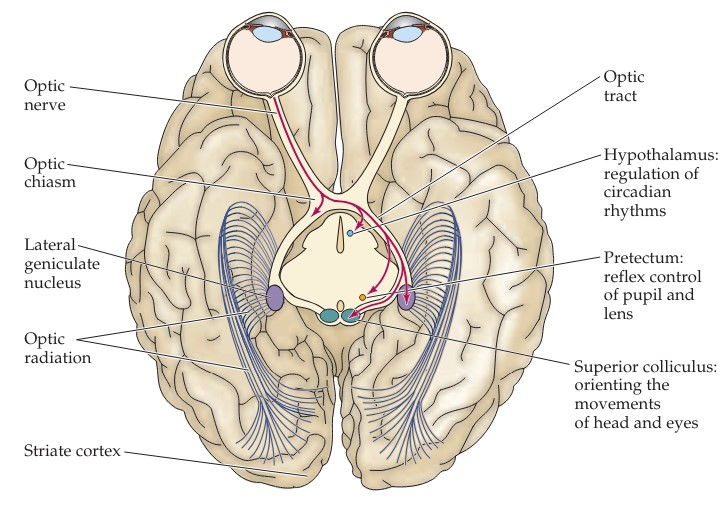
\includegraphics[width=1\textwidth]{Central_Visual_Pathway.jpg}
  \caption{詳細視覺路徑圖~\cite{Purves2004Neuroscience3E}}
  \label{fig:Central_Visual_Pathway}
\end{figure}

\subsubsection{視網膜}

\subsubsection{外側膝狀體}

\subsubsection{視覺皮層}


\subsection{卷積神經網路}

\subsection{以卷積神經網路為基礎的可解釋性深度學習模型}

\section{文獻回顧}

\subsection{可解釋性人工智慧的演進與分類}
Decision Tree:
\cite{rokach2016decision}
\cite{grinsztajn2022treebased}

介紹可解釋性人工智慧的歷程,分類,各分類著名的論文的簡介
可解釋性人工智慧的研究最早可以追蹤到1991年的專家系統時代 W Swartout, C Paris 等人便開始對可解釋性人工智慧進行研究 \cite{87686},
但是

\subsection{對於 Inherently Interpretable 可解釋性模型之研究}
\subsubsection{基於多層自我映射圖之可視覺化深度學習模型}

\subsection{對於 Post-hoc 可解釋性模型之研究}
\subsubsection{Local Interpretable Model-agnostic Explanations(LIME)} 
\subsubsection{Shapley Additive Explanations(SHAP)}

\subsection{近年可解釋性模型趨勢之研究}
\subsubsection{Tabnet: Attentive interpretable tabular learning}
\subsubsection{Building more explainable artificial intelligence with argumentation}
XAI的新趨勢使用論證的方式來解釋,特別是計算論證有助於理解理性決策的所有步驟以及在不確定性下進行推理。 \cite{LONGO2024102301}



\end{document}